\documentclass[1p]{elsarticle_modified}
%\bibliographystyle{elsarticle-num}

%\usepackage[colorlinks]{hyperref}
%\usepackage{abbrmath_seonhwa} %\Abb, \Ascr, \Acal ,\Abf, \Afrak
\usepackage{amsfonts}
\usepackage{amssymb}
\usepackage{amsmath}
\usepackage{amsthm}
\usepackage{scalefnt}
\usepackage{amsbsy}
\usepackage{kotex}
\usepackage{caption}
\usepackage{subfig}
\usepackage{color}
\usepackage{graphicx}
\usepackage{xcolor} %% white, black, red, green, blue, cyan, magenta, yellow
\usepackage{float}
\usepackage{setspace}
\usepackage{hyperref}

\usepackage{tikz}
\usetikzlibrary{arrows}

\usepackage{multirow}
\usepackage{array} % fixed length table
\usepackage{hhline}

%%%%%%%%%%%%%%%%%%%%%
\makeatletter
\renewcommand*\env@matrix[1][\arraystretch]{%
	\edef\arraystretch{#1}%
	\hskip -\arraycolsep
	\let\@ifnextchar\new@ifnextchar
	\array{*\c@MaxMatrixCols c}}
\makeatother %https://tex.stackexchange.com/questions/14071/how-can-i-increase-the-line-spacing-in-a-matrix
%%%%%%%%%%%%%%%

\usepackage[normalem]{ulem}

\newcommand{\msout}[1]{\ifmmode\text{\sout{\ensuremath{#1}}}\else\sout{#1}\fi}
%SOURCE: \msout is \stkout macro in https://tex.stackexchange.com/questions/20609/strikeout-in-math-mode

\newcommand{\cancel}[1]{
	\ifmmode
	{\color{red}\msout{#1}}
	\else
	{\color{red}\sout{#1}}
	\fi
}

\newcommand{\add}[1]{
	{\color{blue}\uwave{#1}}
}

\newcommand{\replace}[2]{
	\ifmmode
	{\color{red}\msout{#1}}{\color{blue}\uwave{#2}}
	\else
	{\color{red}\sout{#1}}{\color{blue}\uwave{#2}}
	\fi
}

\newcommand{\Sol}{\mathcal{S}} %segment
\newcommand{\D}{D} %diagram
\newcommand{\A}{\mathcal{A}} %arc


%%%%%%%%%%%%%%%%%%%%%%%%%%%%%5 test

\def\sl{\operatorname{\textup{SL}}(2,\Cbb)}
\def\psl{\operatorname{\textup{PSL}}(2,\Cbb)}
\def\quan{\mkern 1mu \triangleright \mkern 1mu}

\theoremstyle{definition}
\newtheorem{thm}{Theorem}[section]
\newtheorem{prop}[thm]{Proposition}
\newtheorem{lem}[thm]{Lemma}
\newtheorem{ques}[thm]{Question}
\newtheorem{cor}[thm]{Corollary}
\newtheorem{defn}[thm]{Definition}
\newtheorem{exam}[thm]{Example}
\newtheorem{rmk}[thm]{Remark}
\newtheorem{alg}[thm]{Algorithm}

\newcommand{\I}{\sqrt{-1}}
\begin{document}

%\begin{frontmatter}
%
%\title{Boundary parabolic representations of knots up to 8 crossings}
%
%%% Group authors per affiliation:
%\author{Yunhi Cho} 
%\address{Department of Mathematics, University of Seoul, Seoul, Korea}
%\ead{yhcho@uos.ac.kr}
%
%
%\author{Seonhwa Kim} %\fnref{s_kim}}
%\address{Center for Geometry and Physics, Institute for Basic Science, Pohang, 37673, Korea}
%\ead{ryeona17@ibs.re.kr}
%
%\author{Hyuk Kim}
%\address{Department of Mathematical Sciences, Seoul National University, Seoul 08826, Korea}
%\ead{hyukkim@snu.ac.kr}
%
%\author{Seokbeom Yoon}
%\address{Department of Mathematical Sciences, Seoul National University, Seoul, 08826,  Korea}
%\ead{sbyoon15@snu.ac.kr}
%
%\begin{abstract}
%We find all boundary parabolic representation of knots up to 8 crossings.
%
%\end{abstract}
%\begin{keyword}
%    \MSC[2010] 57M25 
%\end{keyword}
%
%\end{frontmatter}

%\linenumbers
%\tableofcontents
%
\newcommand\colored[1]{\textcolor{white}{\rule[-0.35ex]{0.8em}{1.4ex}}\kern-0.8em\color{red} #1}%
%\newcommand\colored[1]{\textcolor{white}{ #1}\kern-2.17ex	\textcolor{white}{ #1}\kern-1.81ex	\textcolor{white}{ #1}\kern-2.15ex\color{red}#1	}

{\Large $\underline{11a_{190}~(K11a_{190})}$}

\setlength{\tabcolsep}{10pt}
\renewcommand{\arraystretch}{1.6}
\vspace{1cm}\begin{tabular}{m{100pt}>{\centering\arraybackslash}m{274pt}}
\multirow{5}{120pt}{
	\centering
	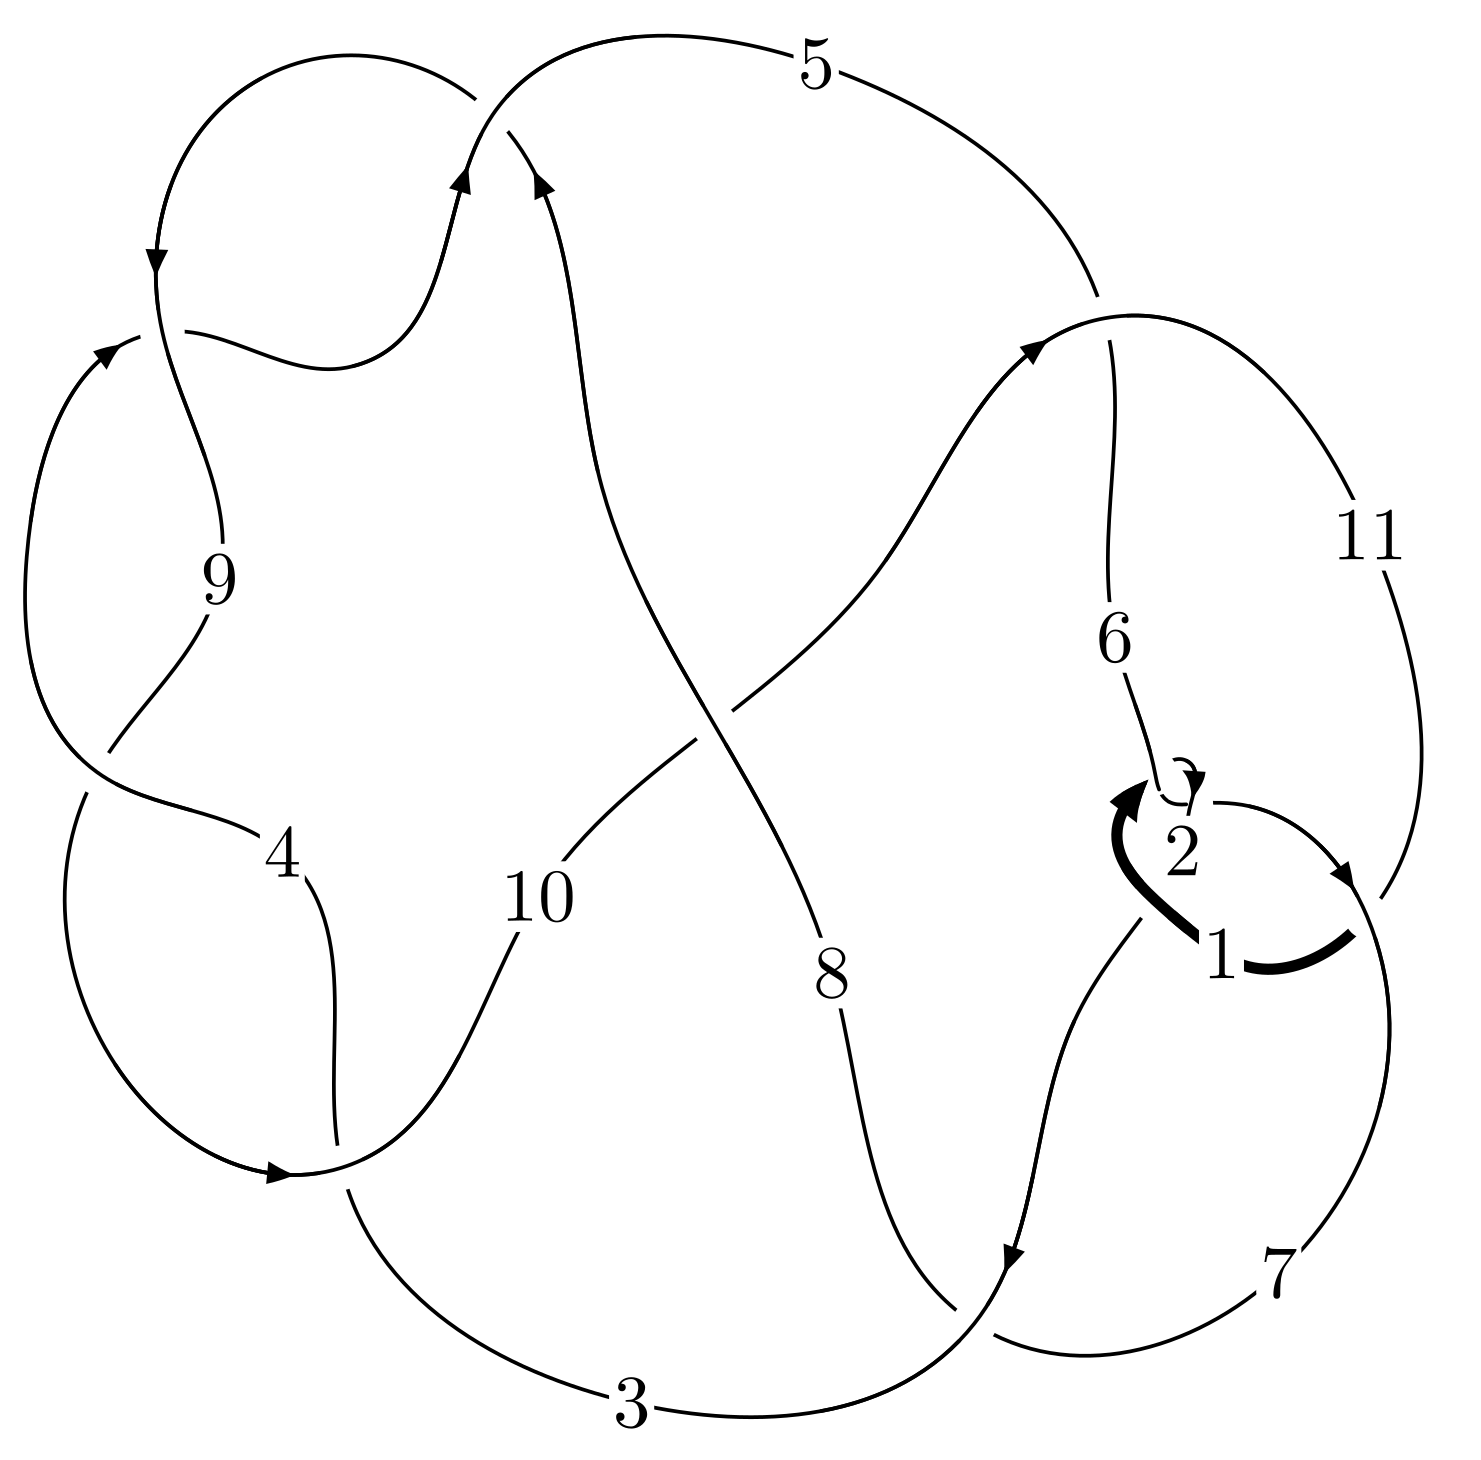
\includegraphics[width=112pt]{../../../GIT/diagram.site/Diagrams/png/439_11a_190.png}\\
\ \ \ A knot diagram\footnotemark}&
\allowdisplaybreaks
\textbf{Linearized knot diagam} \\
\cline{2-2}
 &
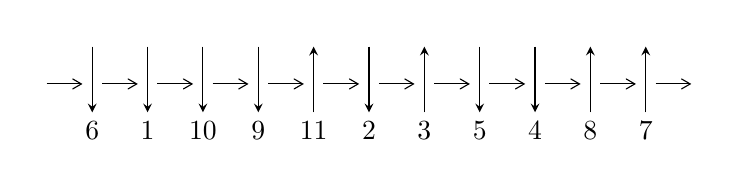
\begin{tikzpicture}[x=20pt, y=17pt]
	% nodes
	\node (C0) at (0, 0) {};
	\node (C1) at (1, 0) {};
	\node (C1U) at (1, +1) {};
	\node (C1D) at (1, -1) {6};

	\node (C2) at (2, 0) {};
	\node (C2U) at (2, +1) {};
	\node (C2D) at (2, -1) {1};

	\node (C3) at (3, 0) {};
	\node (C3U) at (3, +1) {};
	\node (C3D) at (3, -1) {10};

	\node (C4) at (4, 0) {};
	\node (C4U) at (4, +1) {};
	\node (C4D) at (4, -1) {9};

	\node (C5) at (5, 0) {};
	\node (C5U) at (5, +1) {};
	\node (C5D) at (5, -1) {11};

	\node (C6) at (6, 0) {};
	\node (C6U) at (6, +1) {};
	\node (C6D) at (6, -1) {2};

	\node (C7) at (7, 0) {};
	\node (C7U) at (7, +1) {};
	\node (C7D) at (7, -1) {3};

	\node (C8) at (8, 0) {};
	\node (C8U) at (8, +1) {};
	\node (C8D) at (8, -1) {5};

	\node (C9) at (9, 0) {};
	\node (C9U) at (9, +1) {};
	\node (C9D) at (9, -1) {4};

	\node (C10) at (10, 0) {};
	\node (C10U) at (10, +1) {};
	\node (C10D) at (10, -1) {8};

	\node (C11) at (11, 0) {};
	\node (C11U) at (11, +1) {};
	\node (C11D) at (11, -1) {7};
	\node (C12) at (12, 0) {};

	% arrows
	\draw[->,>={angle 60}]
	(C0) edge (C1) (C1) edge (C2) (C2) edge (C3) (C3) edge (C4) (C4) edge (C5) (C5) edge (C6) (C6) edge (C7) (C7) edge (C8) (C8) edge (C9) (C9) edge (C10) (C10) edge (C11) (C11) edge (C12) ;	\draw[->,>=stealth]
	(C1U) edge (C1D) (C2U) edge (C2D) (C3U) edge (C3D) (C4U) edge (C4D) (C5D) edge (C5U) (C6U) edge (C6D) (C7D) edge (C7U) (C8U) edge (C8D) (C9U) edge (C9D) (C10D) edge (C10U) (C11D) edge (C11U) ;
	\end{tikzpicture} \\
\hhline{~~} \\& 
\textbf{Solving Sequence} \\ \cline{2-2} 
 &
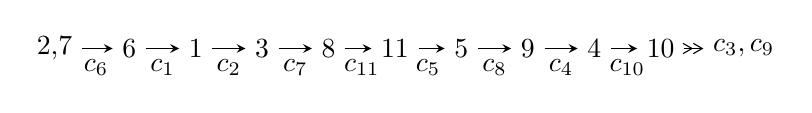
\begin{tikzpicture}[x=24pt, y=7pt]
	% node
	\node (A0) at (-1/8, 0) {2,7};
	\node (A1) at (1, 0) {6};
	\node (A2) at (2, 0) {1};
	\node (A3) at (3, 0) {3};
	\node (A4) at (4, 0) {8};
	\node (A5) at (5, 0) {11};
	\node (A6) at (6, 0) {5};
	\node (A7) at (7, 0) {9};
	\node (A8) at (8, 0) {4};
	\node (A9) at (9, 0) {10};
	\node (C1) at (1/2, -1) {$c_{6}$};
	\node (C2) at (3/2, -1) {$c_{1}$};
	\node (C3) at (5/2, -1) {$c_{2}$};
	\node (C4) at (7/2, -1) {$c_{7}$};
	\node (C5) at (9/2, -1) {$c_{11}$};
	\node (C6) at (11/2, -1) {$c_{5}$};
	\node (C7) at (13/2, -1) {$c_{8}$};
	\node (C8) at (15/2, -1) {$c_{4}$};
	\node (C9) at (17/2, -1) {$c_{10}$};
	\node (A10) at (41/4, 0) {$c_{3},c_{9}$};

	% edge
	\draw[->,>=stealth]	
	(A0) edge (A1) (A1) edge (A2) (A2) edge (A3) (A3) edge (A4) (A4) edge (A5) (A5) edge (A6) (A6) edge (A7) (A7) edge (A8) (A8) edge (A9) ;
	\draw[->>,>={angle 60}]	
	(A9) edge (A10);
\end{tikzpicture} \\ 

\end{tabular} \\

\footnotetext{
The image of knot diagram is generated by the software ``\textbf{Draw programme}" developed by Andrew Bartholomew(\url{http://www.layer8.co.uk/maths/draw/index.htm\#Running-draw}), where we modified some parts for our purpose(\url{https://github.com/CATsTAILs/LinksPainter}).
}\phantom \\ \newline 
\centering \textbf{Ideals for irreducible components\footnotemark of $X_{\text{par}}$} 
 
\begin{align*}
I^u_{1}&=\langle 
u^{42}- u^{41}+\cdots- u+1\rangle \\
\\
\end{align*}
\raggedright * 1 irreducible components of $\dim_{\mathbb{C}}=0$, with total 42 representations.\\
\footnotetext{All coefficients of polynomials are rational numbers. But the coefficients are sometimes approximated in decimal forms when there is not enough margin.}
\newpage
\renewcommand{\arraystretch}{1}
\centering \section*{I. $I^u_{1}= \langle u^{42}- u^{41}+\cdots- u+1 \rangle$}
\flushleft \textbf{(i) Arc colorings}\\
\begin{tabular}{m{7pt} m{180pt} m{7pt} m{180pt} }
\flushright $a_{2}=$&$\begin{pmatrix}0\\u\end{pmatrix}$ \\
\flushright $a_{7}=$&$\begin{pmatrix}1\\0\end{pmatrix}$ \\
\flushright $a_{6}=$&$\begin{pmatrix}1\\- u^2\end{pmatrix}$ \\
\flushright $a_{1}=$&$\begin{pmatrix}u\\- u^3+u\end{pmatrix}$ \\
\flushright $a_{3}=$&$\begin{pmatrix}- u^3\\u^5- u^3+u\end{pmatrix}$ \\
\flushright $a_{8}=$&$\begin{pmatrix}u^8- u^6+u^4+1\\- u^{10}+2 u^8-3 u^6+2 u^4- u^2\end{pmatrix}$ \\
\flushright $a_{11}=$&$\begin{pmatrix}u^3\\- u^3+u\end{pmatrix}$ \\
\flushright $a_{5}=$&$\begin{pmatrix}u^8- u^6+u^4+1\\- u^8+2 u^6-2 u^4\end{pmatrix}$ \\
\flushright $a_{9}=$&$\begin{pmatrix}u^{26}-5 u^{24}+\cdots+u^2+1\\- u^{26}+6 u^{24}+\cdots+2 u^4- u^2\end{pmatrix}$ \\
\flushright $a_{4}=$&$\begin{pmatrix}- u^{39}+8 u^{37}+\cdots+6 u^5-2 u^3\\u^{41}-9 u^{39}+\cdots-3 u^5+u\end{pmatrix}$ \\
\flushright $a_{10}=$&$\begin{pmatrix}- u^{21}+4 u^{19}+\cdots+2 u^3- u\\u^{23}-5 u^{21}+\cdots-3 u^5+u\end{pmatrix}$\\ \flushright $a_{10}=$&$\begin{pmatrix}- u^{21}+4 u^{19}+\cdots+2 u^3- u\\u^{23}-5 u^{21}+\cdots-3 u^5+u\end{pmatrix}$\\&\end{tabular}
\flushleft \textbf{(ii) Obstruction class $= -1$}\\~\\
\flushleft \textbf{(iii) Cusp Shapes $= 4 u^{40}-36 u^{38}+4 u^{37}+168 u^{36}-32 u^{35}-516 u^{34}+136 u^{33}+1152 u^{32}-384 u^{31}-1972 u^{30}+796 u^{29}+2700 u^{28}-1276 u^{27}-3092 u^{26}+1648 u^{25}+3116 u^{24}-1780 u^{23}-2872 u^{22}+1668 u^{21}+2424 u^{20}-1388 u^{19}-1832 u^{18}+1020 u^{17}+1244 u^{16}-640 u^{15}-796 u^{14}+324 u^{13}+484 u^{12}-124 u^{11}-256 u^{10}+28 u^9+112 u^8+8 u^7-48 u^6-20 u^5+24 u^4+16 u^3-8 u^2-2$}\\~\\
\newpage\renewcommand{\arraystretch}{1}
\flushleft \textbf{(iv) u-Polynomials at the component}\newline \\
\begin{tabular}{m{50pt}|m{274pt}}
Crossings & \hspace{64pt}u-Polynomials at each crossing \\
\hline $$\begin{aligned}c_{1},c_{6}\end{aligned}$$&$\begin{aligned}
&u^{42}- u^{41}+\cdots- u+1
\end{aligned}$\\
\hline $$\begin{aligned}c_{2}\end{aligned}$$&$\begin{aligned}
&u^{42}+19 u^{41}+\cdots- u+1
\end{aligned}$\\
\hline $$\begin{aligned}c_{3},c_{4},c_{8}\\c_{9}\end{aligned}$$&$\begin{aligned}
&u^{42}+u^{41}+\cdots+3 u+1
\end{aligned}$\\
\hline $$\begin{aligned}c_{5},c_{7}\end{aligned}$$&$\begin{aligned}
&u^{42}+u^{41}+\cdots-12 u+4
\end{aligned}$\\
\hline $$\begin{aligned}c_{10}\end{aligned}$$&$\begin{aligned}
&u^{42}+13 u^{41}+\cdots+2109 u+283
\end{aligned}$\\
\hline $$\begin{aligned}c_{11}\end{aligned}$$&$\begin{aligned}
&u^{42}-3 u^{41}+\cdots- u+1
\end{aligned}$\\
\hline
\end{tabular}\\~\\
\newpage\renewcommand{\arraystretch}{1}
\flushleft \textbf{(v) Riley Polynomials at the component}\newline \\
\begin{tabular}{m{50pt}|m{274pt}}
Crossings & \hspace{64pt}Riley Polynomials at each crossing \\
\hline $$\begin{aligned}c_{1},c_{6}\end{aligned}$$&$\begin{aligned}
&y^{42}-19 y^{41}+\cdots+y+1
\end{aligned}$\\
\hline $$\begin{aligned}c_{2}\end{aligned}$$&$\begin{aligned}
&y^{42}+9 y^{41}+\cdots-11 y+1
\end{aligned}$\\
\hline $$\begin{aligned}c_{3},c_{4},c_{8}\\c_{9}\end{aligned}$$&$\begin{aligned}
&y^{42}+49 y^{41}+\cdots+y+1
\end{aligned}$\\
\hline $$\begin{aligned}c_{5},c_{7}\end{aligned}$$&$\begin{aligned}
&y^{42}-35 y^{41}+\cdots-328 y+16
\end{aligned}$\\
\hline $$\begin{aligned}c_{10}\end{aligned}$$&$\begin{aligned}
&y^{42}-19 y^{41}+\cdots-701527 y+80089
\end{aligned}$\\
\hline $$\begin{aligned}c_{11}\end{aligned}$$&$\begin{aligned}
&y^{42}+y^{41}+\cdots+37 y+1
\end{aligned}$\\
\hline
\end{tabular}\\~\\
\newpage\flushleft \textbf{(vi) Complex Volumes and Cusp Shapes}
$$\begin{array}{c|c|c}  
\text{Solutions to }I^u_{1}& \I (\text{vol} + \sqrt{-1}CS) & \text{Cusp shape}\\
 \hline 
\begin{aligned}
u &= -0.958451 + 0.182027 I\end{aligned}
 & -1.50976 + 0.22408 I & -7.80723 - 0.81667 I \\ \hline\begin{aligned}
u &= -0.958451 - 0.182027 I\end{aligned}
 & -1.50976 - 0.22408 I & -7.80723 + 0.81667 I \\ \hline\begin{aligned}
u &= -0.794065 + 0.558308 I\end{aligned}
 & \phantom{-}8.84617 + 2.25274 I & \phantom{-}4.58162 - 3.46798 I \\ \hline\begin{aligned}
u &= -0.794065 - 0.558308 I\end{aligned}
 & \phantom{-}8.84617 - 2.25274 I & \phantom{-}4.58162 + 3.46798 I \\ \hline\begin{aligned}
u &= \phantom{-}1.059210 + 0.106332 I\end{aligned}
 & \phantom{-}0.18706 + 2.88066 I & -2.91592 - 4.70329 I \\ \hline\begin{aligned}
u &= \phantom{-}1.059210 - 0.106332 I\end{aligned}
 & \phantom{-}0.18706 - 2.88066 I & -2.91592 + 4.70329 I \\ \hline\begin{aligned}
u &= \phantom{-}0.534293 + 0.761914 I\end{aligned}
 & \phantom{-}13.9445 - 3.9233 I & \phantom{-}5.91216 + 2.83813 I \\ \hline\begin{aligned}
u &= \phantom{-}0.534293 - 0.761914 I\end{aligned}
 & \phantom{-}13.9445 + 3.9233 I & \phantom{-}5.91216 - 2.83813 I \\ \hline\begin{aligned}
u &= \phantom{-}0.814354 + 0.428559 I\end{aligned}
 & \phantom{-}1.05337 - 1.87068 I & \phantom{-}3.39079 + 4.68483 I \\ \hline\begin{aligned}
u &= \phantom{-}0.814354 - 0.428559 I\end{aligned}
 & \phantom{-}1.05337 + 1.87068 I & \phantom{-}3.39079 - 4.68483 I \\ \hline\begin{aligned}
u &= \phantom{-}0.437218 + 0.793916 I\end{aligned}
 & \phantom{-}13.4042 + 6.9529 I & \phantom{-}5.22220 - 3.15637 I \\ \hline\begin{aligned}
u &= \phantom{-}0.437218 - 0.793916 I\end{aligned}
 & \phantom{-}13.4042 - 6.9529 I & \phantom{-}5.22220 + 3.15637 I \\ \hline\begin{aligned}
u &= -0.510362 + 0.737623 I\end{aligned}
 & \phantom{-}5.58647 + 2.00252 I & \phantom{-}4.43798 - 4.06646 I \\ \hline\begin{aligned}
u &= -0.510362 - 0.737623 I\end{aligned}
 & \phantom{-}5.58647 - 2.00252 I & \phantom{-}4.43798 + 4.06646 I \\ \hline\begin{aligned}
u &= -1.109120 + 0.092741 I\end{aligned}
 & \phantom{-}8.15110 - 4.89812 I & -0.84749 + 2.79086 I \\ \hline\begin{aligned}
u &= -1.109120 - 0.092741 I\end{aligned}
 & \phantom{-}8.15110 + 4.89812 I & -0.84749 - 2.79086 I \\ \hline\begin{aligned}
u &= -0.440224 + 0.767604 I\end{aligned}
 & \phantom{-}5.20119 - 4.76095 I & \phantom{-}3.47757 + 4.70504 I \\ \hline\begin{aligned}
u &= -0.440224 - 0.767604 I\end{aligned}
 & \phantom{-}5.20119 + 4.76095 I & \phantom{-}3.47757 - 4.70504 I \\ \hline\begin{aligned}
u &= -1.052970 + 0.403941 I\end{aligned}
 & -2.94816 + 1.84155 I & -7.97014 - 0.12089 I \\ \hline\begin{aligned}
u &= -1.052970 - 0.403941 I\end{aligned}
 & -2.94816 - 1.84155 I & -7.97014 + 0.12089 I \\ \hline\begin{aligned}
u &= \phantom{-}1.079910 + 0.334044 I\end{aligned}
 & \phantom{-}3.19579 - 0.38496 I & -4.05769 + 0.70837 I \\ \hline\begin{aligned}
u &= \phantom{-}1.079910 - 0.334044 I\end{aligned}
 & \phantom{-}3.19579 + 0.38496 I & -4.05769 - 0.70837 I \\ \hline\begin{aligned}
u &= \phantom{-}0.460288 + 0.731314 I\end{aligned}
 & \phantom{-}3.06576 + 1.25733 I & -0.386808 - 0.265317 I \\ \hline\begin{aligned}
u &= \phantom{-}0.460288 - 0.731314 I\end{aligned}
 & \phantom{-}3.06576 - 1.25733 I & -0.386808 + 0.265317 I \\ \hline\begin{aligned}
u &= \phantom{-}1.069990 + 0.454007 I\end{aligned}
 & -2.58903 - 5.04565 I & -5.96481 + 8.68441 I \\ \hline\begin{aligned}
u &= \phantom{-}1.069990 - 0.454007 I\end{aligned}
 & -2.58903 + 5.04565 I & -5.96481 - 8.68441 I \\ \hline\begin{aligned}
u &= -1.096730 + 0.488278 I\end{aligned}
 & \phantom{-}4.21047 + 6.88158 I & -1.95632 - 6.72572 I \\ \hline\begin{aligned}
u &= -1.096730 - 0.488278 I\end{aligned}
 & \phantom{-}4.21047 - 6.88158 I & -1.95632 + 6.72572 I \\ \hline\begin{aligned}
u &= -1.049770 + 0.605621 I\end{aligned}
 & \phantom{-}3.98383 + 3.11596 I & \phantom{-}2.01311 - 1.17218 I \\ \hline\begin{aligned}
u &= -1.049770 - 0.605621 I\end{aligned}
 & \phantom{-}3.98383 - 3.11596 I & \phantom{-}2.01311 + 1.17218 I\\
 \hline 
 \end{array}$$\newpage$$\begin{array}{c|c|c}  
\text{Solutions to }I^u_{1}& \I (\text{vol} + \sqrt{-1}CS) & \text{Cusp shape}\\
 \hline 
\begin{aligned}
u &= \phantom{-}1.042540 + 0.627034 I\end{aligned}
 & \phantom{-}12.43060 - 1.33379 I & \phantom{-}3.69918 + 2.21003 I \\ \hline\begin{aligned}
u &= \phantom{-}1.042540 - 0.627034 I\end{aligned}
 & \phantom{-}12.43060 + 1.33379 I & \phantom{-}3.69918 - 2.21003 I \\ \hline\begin{aligned}
u &= \phantom{-}1.074510 + 0.592401 I\end{aligned}
 & \phantom{-}1.24809 - 6.31321 I & -3.41953 + 4.87109 I \\ \hline\begin{aligned}
u &= \phantom{-}1.074510 - 0.592401 I\end{aligned}
 & \phantom{-}1.24809 + 6.31321 I & -3.41953 - 4.87109 I \\ \hline\begin{aligned}
u &= -1.091090 + 0.602467 I\end{aligned}
 & \phantom{-}3.27056 + 9.94153 I & \phantom{-}0.33743 - 9.11948 I \\ \hline\begin{aligned}
u &= -1.091090 - 0.602467 I\end{aligned}
 & \phantom{-}3.27056 - 9.94153 I & \phantom{-}0.33743 + 9.11948 I \\ \hline\begin{aligned}
u &= \phantom{-}1.100260 + 0.611942 I\end{aligned}
 & \phantom{-}11.4291 - 12.2349 I & \phantom{-}2.31503 + 7.47393 I \\ \hline\begin{aligned}
u &= \phantom{-}1.100260 - 0.611942 I\end{aligned}
 & \phantom{-}11.4291 + 12.2349 I & \phantom{-}2.31503 - 7.47393 I \\ \hline\begin{aligned}
u &= -0.194284 + 0.626683 I\end{aligned}
 & \phantom{-}6.70392 - 2.62174 I & \phantom{-}1.89600 + 2.88322 I \\ \hline\begin{aligned}
u &= -0.194284 - 0.626683 I\end{aligned}
 & \phantom{-}6.70392 + 2.62174 I & \phantom{-}1.89600 - 2.88322 I \\ \hline\begin{aligned}
u &= \phantom{-}0.124492 + 0.489748 I\end{aligned}
 & -0.169198 + 1.278750 I & -1.95713 - 5.54449 I \\ \hline\begin{aligned}
u &= \phantom{-}0.124492 - 0.489748 I\end{aligned}
 & -0.169198 - 1.278750 I & -1.95713 + 5.54449 I\\
 \hline 
 \end{array}$$\newpage
\newpage\renewcommand{\arraystretch}{1}
\centering \section*{ II. u-Polynomials}
\begin{tabular}{m{50pt}|m{274pt}}
Crossings & \hspace{64pt}u-Polynomials at each crossing \\
\hline $$\begin{aligned}c_{1},c_{6}\end{aligned}$$&$\begin{aligned}
&u^{42}- u^{41}+\cdots- u+1
\end{aligned}$\\
\hline $$\begin{aligned}c_{2}\end{aligned}$$&$\begin{aligned}
&u^{42}+19 u^{41}+\cdots- u+1
\end{aligned}$\\
\hline $$\begin{aligned}c_{3},c_{4},c_{8}\\c_{9}\end{aligned}$$&$\begin{aligned}
&u^{42}+u^{41}+\cdots+3 u+1
\end{aligned}$\\
\hline $$\begin{aligned}c_{5},c_{7}\end{aligned}$$&$\begin{aligned}
&u^{42}+u^{41}+\cdots-12 u+4
\end{aligned}$\\
\hline $$\begin{aligned}c_{10}\end{aligned}$$&$\begin{aligned}
&u^{42}+13 u^{41}+\cdots+2109 u+283
\end{aligned}$\\
\hline $$\begin{aligned}c_{11}\end{aligned}$$&$\begin{aligned}
&u^{42}-3 u^{41}+\cdots- u+1
\end{aligned}$\\
\hline
\end{tabular}\newpage\renewcommand{\arraystretch}{1}
\centering \section*{ III. Riley Polynomials}
\begin{tabular}{m{50pt}|m{274pt}}
Crossings & \hspace{64pt}Riley Polynomials at each crossing \\
\hline $$\begin{aligned}c_{1},c_{6}\end{aligned}$$&$\begin{aligned}
&y^{42}-19 y^{41}+\cdots+y+1
\end{aligned}$\\
\hline $$\begin{aligned}c_{2}\end{aligned}$$&$\begin{aligned}
&y^{42}+9 y^{41}+\cdots-11 y+1
\end{aligned}$\\
\hline $$\begin{aligned}c_{3},c_{4},c_{8}\\c_{9}\end{aligned}$$&$\begin{aligned}
&y^{42}+49 y^{41}+\cdots+y+1
\end{aligned}$\\
\hline $$\begin{aligned}c_{5},c_{7}\end{aligned}$$&$\begin{aligned}
&y^{42}-35 y^{41}+\cdots-328 y+16
\end{aligned}$\\
\hline $$\begin{aligned}c_{10}\end{aligned}$$&$\begin{aligned}
&y^{42}-19 y^{41}+\cdots-701527 y+80089
\end{aligned}$\\
\hline $$\begin{aligned}c_{11}\end{aligned}$$&$\begin{aligned}
&y^{42}+y^{41}+\cdots+37 y+1
\end{aligned}$\\
\hline
\end{tabular}
\vskip 2pc
\end{document}